\chapter{Árbol Generador Mínimo}

\section{Definición}

\subsubsection{Grafos pesados}

Un \textit{grafo pesado} es un grafo $G = (V, E)$ junto con una función $w: E \longrightarrow \N$, donde $w(e)$ es el peso de la arista $e$. El peso suele usarse para modelar diversas magnitudes, como el costo de una arista, o tiempo que se tarda en pasar por ella.

% TODO: Imagen

\subsubsection{AGM}

Un \textit{árbol generador mínimo} (AGM) es un \hyperref[arbol-generador]{árbol generador} cuyo peso total es menor al de todos los demás AGs, donde peso total se define como la suma de los pesos de sus aristas. Formalmente, el problema es el siguiente:

\begin{problema}
    Dado un grafo $G = (V, E)$ y una función de peso $w: E \longrightarrow \N$, encontrar un AG $T = (V, E_T)$ que cumpla:
    $$w(T) = \sum_{e \in E_T} w(e) \leq \sum_{e \in E_{T'}} w(e) = w(T')$$

    Para cualquier árbol generador $T' = (V, E_{T'})$ en $G$.
\end{problema}

También se puede definir el árbol generador máximo, que maximiza el peso total de $T$, pero este problema se puede \hyperref[reducciones]{reducir} al anterior: si se toman los pesos $w'(e) = -w(e)$, el peso  de cualquier AG $T$ será $w'(T) = \sum_{e \in E_T} w'(e) = \sum_{e \in E_T} -w(e) = -w(T)$, y por ende:
\begin{align*}
    w'(AGM) \leq w'(T) & \iff -w'(AGM) \geq -w'(T) \\
                       & \iff w(AGM) \geq w(T)
\end{align*}

\subsubsection{Propiedades}

El AGM de un grafo \underline{no necesariamente es único}: pueden varios grafos con el mismo peso, que es menor al de todos los demás.

\begin{figure}[H]
    \centering
    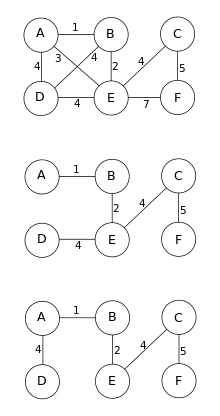
\includegraphics[width=0.3\textwidth]{ejemplo_agm.png}
    \caption*{Un grafo y 2 de sus AGMs, ambos con peso total $16$.}
\end{figure}

\subsubsection{Algoritmos}

En las siguientes secciones analizaremos $2$ algoritmos para encontrar un AGM: el algoritmo de Prim y el de Kruskal. Ambos son golosos: siguen estrategias que toman en cada paso la mejor decisión a corto plazo, y en este caso devuelven soluciones óptimas. Logran esto armando progresivamente un bosque (en el caso de Prim un árbol) en un ciclo que mantiene el invariante de que sus aristas forman un subconjunto de las de algún AGM.

\begin{codebox}
    \Procname{$\proc{Arbol-Generador-Minimo}(G, w)$}
    \li Inicializar grafo $T = (V, \emptyset)$
    \li \While $T$ no es un AG (es disconexo): \Do
    \li Encontrar una arista segura $e$.
    \li Agregar $e$ a $E_T$.
    \End
    \li \Return $T$
\end{codebox}

\label{arista-segura}
En este contexto una arista es \textit{segura} cuando se puede agregar al bosque $T$ y mantener el invariante (es un subconjunto de algún AGM). Encontrar una es donde radica la dificultad del problema, y es en donde difieren los algoritmos.

\section{Algoritmo de Prim}

\subsection{Introducción}

El \textit{algoritmo de Prim} mantiene un árbol $T = (V_T, E_T)$, y en cada iteración agrega un nuevo vértice de $V - V_T$ al mismo (junto con una arista a $E_T$), hasta que $T$ pasa por todos los vértices de $G$ (y se vuelve un AG). La arista seleccionada en cada paso es la de mínimo peso entre todas las $(u, v) \in V_T \times (V - V_T)$ (las que conectan vértices dentro del árbol con los de afuera).

Se puede implementar de la siguiente manera:

\begin{codebox}
    \Procname{$\proc{Prim}(G, w)$}
    \li $V_T \gets \{s\}$ (cualquier vértice)
    \li $E_T \gets \emptyset$
    \li \For $i \gets 1$ \To $n - 1$ \Do
    \li $e \gets \arg\min{\{w(e) \mid e = uv \in E,\ u \in V_T,\ v \in V - V_T\}}$
    \li $E_T \gets E_T \cup e$
    \li $V_T \gets V_T \cup v$
    \End
    \li \Return $T \gets (V_T, E_T)$
\end{codebox}

El algoritmo asume que el grafo es conexo. Si esto no se cumple, se puede modificar el algoritmo levemente\footnote{El único problema que tiene esa implementación es que asume que el conjunto del que se toma el $\arg\min$ no está vacío. Si esto se chequea en cada iteración, se puede terminar la ejecución cuando no quedan vértices por agregar.} para que devuelva el AGM de la componente conexa que contiene al vértice inicial.

\subsection{Correctitud}

\begin{theorem*}
    El árbol que devuelve el algoritmo de Prim es un AGM.
\end{theorem*}
\begin{proof}
    Se demuestra por inducción. La hipótesis inductiva será la siguiente: $\forall\,0 \leq k \leq n - 1, T_k = (V_k, E_k)$, el grafo mantenido por Prim en la $k$-ésima iteración del ciclo, es un árbol y es subgrafo de algún AGM de $G$.

    \textbf{Caso Base}: En el paso $k = 0$, todavía no se entró al ciclo, así que $T_0 = (\{s\}, \emptyset)$, que es un árbol (no tiene ciclos) y es subgrafo de cualquier AG (y por lo tanto de cualquier AGM).

    \textbf{Paso Inductivo}: Sea $e = vw$ agregada en la iteración. Luego, $T_k = (V_k, E_k) = (V_{k - 1} \cup \{w\}, E_{k - 1} \cup \{e\})$. Por hipótesis inductiva, se sabe que $T_{k - 1}$ es subgrafo de algún árbol generador $T$. Existen dos posibilidades:
    \begin{itemize}
        \item $e \in E_T$, en cuyo caso $T_k$ es también subgrafo de $T$.
        \item $e \notin E_T$. Aún así, sabemos que $V_{k - 1}$ forma una componente conexa en $T$, porque $T_{k - 1}$ es un subgrafo suyo y es conexo (es un árbol). Entonces, debe haber alguna arista $e' = v'w' \in E_T$ que conecta $V_{k - 1}$ y $V - V_{k - 1}$. Si se saca esa arista de $T$, las componentes se vuelven disconexas, pero se pueden volver a conectar usando la arista $e$.

              Por ende, $T' = T + e - e' = (V, (E_T \cup \{e\}) - \{e'\})$ es un árbol (y es generador, ya que contiene a todos los vértices). Además, como $e'$ era una de las aristas que se podían elegir al principio de la iteración (conecta a $V_{k - 1}$ con $V - V_{k - 1}$), se debe cumplir que $w(e) \leq w(e')$, así que:
              $$w(T') = w(T) + \underbrace{w(e) - w(e')}_{\leq 0} \leq w(T)$$

              Por lo tanto, el peso total de $T'$ es menor o igual al de un AGM, así que este también es AGM. Como $T_k$ es subgrafo de $T'$ ($E_k = E_{k - 1} \cup \{e\} \subseteq E_T \cup \{e\}, e' \notin E_k$), se cumple la propiedad.
    \end{itemize}

    Dado que la propiedad vale al terminar cualquier iteración, también se cumple en $k = n - 1$, donde $T_{k - 1}$ tiene $n$ vértices, y por lo tanto es un árbol generador (y mínimo).

\end{proof}

\subsection{Complejidad}
\label{complejidad-prim}

Para implementar el algoritmo de Prim, es necesario determinar un método para encontrar la arista de menor peso entre $V_T$ y $V - V_T$. Esto se puede lograr utilizando una cola de prioridad, pero la forma en la que esta se represente puede variar:
\begin{itemize}
    \item \underline{Un arreglo de $|V|$ posiciones}: En este caso, el peso de la arista que conecta a cada vértice con el árbol se guarda en una posición del arreglo (los vértices que ya se agregaron se marcan con un valor especial). Para determinar el siguiente vértice a agregar, se toma el mínimo del arreglo, y una vez que se agrega se actualizan las posiciones correspondientes (en caso de que uno de sus vecinos se pueda alcanzar con peso menor al anterior). Ambas operaciones son \BigO{|V|}, y como se realizan $|V| - 1$ operaciones, la complejidad total \BigO{|V|^2}.
    \item \underline{Un heap}: En este caso, se mantiene un mín-heap de los nodos que no fueron explorados, donde la clave es el peso mínimo entre las aristas que lo conectan al árbol. En cada paso se desencola un vértice, y se actualizan las claves de sus vecinos\footnote{Para lograr esto en tiempo logarítmico, es preferible usar un árbol balanceado (como los AVLs) antes que un heap.}. Esto implica que se realizan $1 + d(v)$ operaciones logarítmicas en cada iteración, lo cual resulta en una complejidad total de \BigO{(|V| + |E|)\log{|V|}}. Como se asume que $G$ es conexo, $|E| \geq |V| - 1$, y por ende $\BigO{(|V| + |E|)\log{|V|}} \subseteq \BigO{|E|\log{|V|}}$.
\end{itemize}

En el caso de los grafos \textit{densos}, que se podrían definir como aquellos en los que $|E| \in \BigOmega{|V|^2}$, la segunda alternativa tendría complejidad \BigO{|V|^2\log{|V|}}, mientras que la primera solo \BigO{|V|^2}. Por otro lado, si el grafo es \textit{ralo}, que sería cuando $|E| \in \BigO{|V|}$, la segunda sería tan solo \BigO{|V|\log{|V|}}, mejor que \BigO{|V^2|}.

Hay una tercera opción para representar la cola de prioridad: a través de Fibonacci heaps. Estos permiten que el algoritmo corra en \BigO{|E| + |V|\log{|V|}} (asintóticamente mejor que las dos anteriores), pero es más complejo de implementar que las otras opciones.

\section{Algoritmo de Kruskal}

\subsection{Disjoint-Set/Union-Find}

Antes de ver el algoritmo en sí, es necesario una de las estructuras que usa: el \textit{Disjoint-Set} o \textit{Union-Find}. Esta mantiene una partición $P_1, ..., P_n$ de un conjunto $C$, asignándole a todos los elementos de cada $P_i$ un mismo representante $r_i$. Permite realizar las siguientes operaciones de forma eficiente:
\begin{itemize}
    \item \proc{Make-Set}($x$): crea un nuevo conjunto $\{x\}$ dentro de la partición. Como precondición, $x$ no puede estar en ninguno de los conjuntos anteriores.
    \item \proc{Union}($x$, $y$): Reemplaza los conjuntos que contenían a $x$ e $y$, $S_x, S_y$ por su unión $S_x \cup S_y$.
    \item \proc{Find}($x$): Devuelve el representante $r_x$ de $x$ dentro de la partición. Esto puede ser utilizado para comprobar si dos elementos pertenecen al mismo conjunto.
\end{itemize}

\subsubsection{Implementación}

Internamente, la estructura se implementa como un bosque, donde cada árbol se corresponde con el conjunto de la partición que contiene a sus vértices, y la raíz es el representante. Implementar la operación \proc{Union} es simple: solo es necesario agregar a la raíz de uno de los conjuntos como hijo de la raíz del otro. \proc{Find} también resulta trivial: solo es necesario recorrer los antecesores de cada nodo hasta llegar a la raíz.

Esto alcanza para implementar a la estructura, pero la complejidad no es ideal: los árboles podrían ser degenerados (una línea donde cada nodo tiene $1$ solo hijo), lo cual haría que \proc{Find} sea \BigO{n}. Para evitar que suceda esto, se emplean 2 heurísticas:
\begin{itemize}
    \item \textbf{Union by rank}\footnote{Es equivalente usar la alternativa \textbf{union by size}, que usa la cantidad de nodos en el árbol en lugar de la altura.}: Esto implica mantener la altura de cada árbol guardado, lo cual en este caso no es costoso: la única forma en la que puede cambiar es cuando se agrega otro árbol $T$ a la raíz como hijo, y en tal caso la altura pasa a ser el mínimo entre la anterior y $h(T) + 1$. Esto se utiliza a la hora de decidir qué raíz utilizar para el nuevo árbol de \proc{Union}: se elige la que resulte en menor altura (queda como raíz el representante de mayor rango).
    \item \textbf{Path compression}: Esta optimización se basa en el hecho de que la estructura interna del árbol no es rígida: solo se debe cumplir que la raíz sea el representante de todos los nodos. Por ende, cada vez que se realiza un \proc{Find}, todos los vértices transitados se pueden colocar como hijos directos del árbol.
\end{itemize}

Los algoritmos se pueden implementar de la siguiente manera, donde \id{prev} es el arreglo que guarda los antecesores de cada nodo (representa al bosque) y \id{rank}[$v$] guarda la altura del árbol con raíz en $v$:
\begin{codebox}
    \Procname{$\proc{Make-Set}(x)$}
    \li $\id{prev}[x] \gets x$
    \li $\id{rank}[x] \gets 0$
\end{codebox}
\begin{codebox}
    \Procname{$\proc{Union}(x, y)$}
    \li $r_x \gets \proc{Find}(x), r_y \gets \proc{Find}(y)$
    \li \If $\id{rank}[r_x] > \id{rank}[r_y]$ \Then
    \li $\id{prev}[y] = x$
    \li \Else
    \li $\id{prev}[x] = y$
    \li \If $\id{rank}[x] == \id{rank}[y]$ \Then
    \li $\id{rank}[y] \gets \id{rank}[y] + 1$
    \End
    \End
\end{codebox}
\begin{codebox}
    \Procname{$\proc{Find}(x)$}
    \li \If $x \neq \id{prev}[x]$ \Then
    \li $\id{prev}[x] \gets \proc{Find}(\id{prev}[x])$
    \End
    \li \Return $\id{prev}[x]$
\end{codebox}

Haciendo uso de ambas heurísticas, la complejidad de peor caso amortizada de la operación \proc{Find} (y por ende también la de \proc{Union}) baja a \BigO{\alpha(n)}, donde $\alpha$ es la función de Ackermann inversa\footnote{A efectos prácticos, $\alpha(n) \leq 5$}.

\subsection{Algoritmo}

Teniendo esta estructura, se puede definir el \textit{algoritmo de Kruskal}: se construye un bosque, recorriendo todas las aristas en orden de peso creciente, y mientras tanto se mantiene un Union-Find con las componentes conexas del bosque. Cada vez que se visita una arista, se chequea si conecta dos vértices de componentes conexas distintas. Si es así, se corre \proc{Union} sobre los conjuntos de las componentes, y la arista es agregada al árbol. Esto se hace hasta que queda una sola componente, y queda formado un árbol generador (que además es mínimo).

\begin{codebox}
    \Procname{$\proc{Kruskal}(G, w)$}
    \li $T \gets (V, E_T \gets \emptyset)$
    \li \For \Each $v \in V$ \Do
    \li $\proc{Make-Set}(v)$
    \End
    \li \For \Each $uv \in E_T$, en orden de $w$ creciente \Do
    \li \If $\proc{Find}(u) \neq \proc{Find}(v)$ \Then
    \li $E_T \gets E_T \cup {uv}$
    \li $\proc{Union}(u, v)$
    \End
    \li \Return $T$
\end{codebox}

\subsection{Correctitud}

La correctitud de este algoritmo se puede demostrar de forma similar al anterior:
\begin{theorem*}
    El árbol que devuelve el algoritmo de Kruskal es un AGM.
\end{theorem*}
\begin{proof}
    Se demuestra por inducción con la siguiente hipótesis inductiva: $\forall\,0 \leq k \leq n - 1, T_k = (V_k, E_k)$, el grafo mantenido por Kruskal después de agregar la $k$-ésima arista, es un bosque y subgrafo de algún AGM de $G$.

    \textbf{Caso Base}: En $k = 0$, el grafo es $T_0 = (V, \emptyset)$, que es subgrafo de cualquier AG, y no tiene ciclos (así que es un bosque).

    \textbf{Paso Inductivo}: Sea $uv \in E$ la $k$-ésima arista agregada al grafo. Por hipótesis inductiva, sabemos que $T_{k - 1}$ es un bosque, y como las aristas deben conectar componentes distintas, la nueva arista no forma parte de ningún ciclo, así que $T_k$ sigue siendo un bosque.

    Por otro lado, la HI también implica que $T_{k - 1}$ es subgrafo de algún AGM $T$. Como los árboles son conexos, debe haber algún camino de $T$ entre los vértices $u$ y $v$. Si este camino es solo la arista $uv$, $T_k$ también es un subgrafo del árbol. Por otro lado, si el camino es distinto, seguro contiene una arista $u'v'$ que conectaría el componente de $u$ en $T_{k - 1}$ con algún otro (porque $v$ no es alcanzable desde $u$ en $T_{k - 1}$). Eso implica que $w(uv) \leq w(u'v')$, ya que $uv$ es la arista de menor peso que cumple esa propiedad.

    Si se toma $T' = (V, (E \cup \{uv\} - \{u'v'\}))$, $T'$ es un árbol porque agregar $uv$ genera un único ciclo que contiene a $u'v'$, y sacar esta arista lo rompe. Por otro lado, su peso es:
    $$w(T') = w(T) + \underbrace{w(uv) - w(u'v')}_{\leq 0} \leq w(T)$$

    Por ende, $T'$ es un AGM y, como $T_k$ es un subgrafo de $T'$, se cumple la propiedad.

\end{proof}

\subsection{Complejidad}

El algoritmo de Kruskal tiene dos pasos generales: ordenar las aristas, y recorrerlas hasta armar el árbol. El ordenamiento es una operación \BigO{|E|\log{|E|}}, mientras que el ciclo realiza a lo sumo $|E|$ iteraciones, y en cada se hace una llamada a \proc{Union}, que tiene complejidad \BigO{\alpha{|V|}}. Aprovechando que $|E| \in \BigO{|V|^2}$, se tiene $\BigO{|E|\log{|E|}} \subseteq \BigO{|E|\log{(|V|^2)}} = \BigO{|E|\log{|V|}}$. La complejidad final entonces es:
$$\BigO{|E|\log{|V|} + |E|\alpha(|V|)} = \BigO{|E|\log{|V|}}$$

\section{Camino Minimáx}

\subsection{Definición}

Dado un grafo pesado $G = (V, E)$ con $w: E \longrightarrow \N$, el \textit{camino minimáx} entre un par de vértices $u, v \in V$ es aquel que minimiza el peso de la arista más pesada del camino. Formalmente, es el $P_m$ que cumple:
$$P_m = \arg\min{\{\max{\{w(e) \mid e \in P\}} \mid P \text{ camino entre $u$ y $v$}\}}$$

Análogamente, el camino maximín es aquél que maximiza el peso de la arista menos pesada del camino, es decir, el $P_M$ tal que:
$$P_M = \arg\max{\{\min{\{w(e) \mid e \in P\}} \mid P \text{ camino entre $u$ y $v$}\}}$$

% TODO: Imagen

Esta noción tiene varias aplicaciones: en general se la conoce como ``ancho de banda''. Podría utilizarse para modelar la cantidad de datos que se pueden transmitir entre dos terminales pasando por una red con ciertas capacidades\footnote{Con la restricción de que todos los datos pasan por un mismo camino; si se pueden ``dividir'', es un problema de \hyperref[flujo]{flujo}.}, o la cantidad de peso que puede pasar por una red de puentes con límites dados.

\subsection{Solución}

El método para encontrar un camino minimax entre dos vértices es simple:
\begin{theorem*}
    Dado un grafo pesado $G = (V, E)$ con $w: E \longrightarrow \N$ y un AGM $T$, para cualquier par de vértices $u,v \in V$, el camino que conecta a $u$ con $v$ en $T$ es minimax.
\end{theorem*}
\begin{proof}
    Supongamos que existe un camino minimax $P$ que pasa por aristas que no están en el árbol $T$. Sea $uv \in E \cap P - E_T$, y $T_{uv}$ el camino que conecta sus vértices en el árbol. Luego, si se toma $e' = \arg\max{\{w(e) \mid e \in T_{uv}\}}$, se puede ver que $w(uv) \geq w(e')$, ya que si no $e'$ podría ser reemplazada por $uv$, formando un AG $T \cup \{uv\} - \{e'\}$ con un peso estrictamente menor, lo cual es absurdo porque $T$ es AGM.

    Por ende, cualquier arista fuera del árbol puede ser reemplazada por un camino que pasa por el árbol y tiene aristas de menor o igual peso (así que el peso máximo del camino se mantiene igual). Entonces, queda demostrado que siempre existe un camino minimáx que pasa por el árbol.

\end{proof}

Esto significa que, para encontrar el camino minimáx entre cualquier par de vértices, se puede calcular el AGM del grafo, y tomar el camino que los une dentro de este. Para el camino maximín, se puede tomar el árbol generador máximo (la demostración es análoga).
